\documentclass[a4paper,12pt]{article} % тип документа

% Поля страниц
\usepackage[left=2.5cm,right=2.5cm,top=2cm,bottom=2cm,bindingoffset=0cm]{geometry}
    
% Отступ после заголовка
\usepackage{indentfirst}

% Картинки
\usepackage{graphicx}

% Таблицы
\usepackage{booktabs}

% Русский язык
\usepackage{cmap}  % поиск в PDF
\usepackage{mathtext}  % русские буквы в формулах
\usepackage[T2A]{fontenc}  % кодировка
\usepackage[utf8]{inputenc}  % кодировка исходного текста
\usepackage[english,russian]{babel}  % локализация и переносы

% Математика
\usepackage{amsmath}

% Ссылки TODO
% \usepackage[unicode=true]{hyperref}
% \usepackage[T1]{fontenc}


\begin{document}

\begin{center}   
	\large{Лабораторная работа № 2.5.1\\\textbf{Измерение коэффициента поверхностного натяжения жидкости}}\\
\end{center}

\section{Аннотация}

\noindent\textbf{Цель работы:}
1) измерение температурной зависимости  коэффициента поверхностного натяжения дистиллированной воды с использованием известного коэффициента поверхностного натяжения спирта; 2) определение полной поверхностной энергии  и теплоты, необходимой для изотермического образования единицы  поверхности жидкости  при различной температуре.
	
\bigskip
\noindent\textbf{В работе используются:} прибор  Ребиндера  с термостатом и микроманометром; исследуемые жидкости; стаканы; микроскоп.

\section{Теоретические сведения}

Наличие поверхностного слоя приводит к различию давлений по разные стороны от искривленной границы раздела двух сред.  Для сферического пузырька с воздухом  внутри жидкости избыточное давление даётся формулой Лапласа:

\begin{equation}\label{лаплас}
\Delta P = P_{внутри}- P_{снаружи}=\frac{2\sigma}{r}, 
\end{equation}
где $\sigma$ -- коэффициент поверхностного натяжения, $P_{внутри}$ и $Р_{снаружи}$ -- давление внутри пузырька и снаружи, $r$ -- радиус кривизны поверхности раздела двух фаз. Эта формула лежит в основе предлагаемого метода определения коэффициента поверхностного натяжения жидкости. Измеряется давление $\Delta P$, необходимое для выталкивания в жидкость пузырька воздуха.

\newpage

\section{Используемое оборудование}

\begin{figure}[h!]
\begin{center}
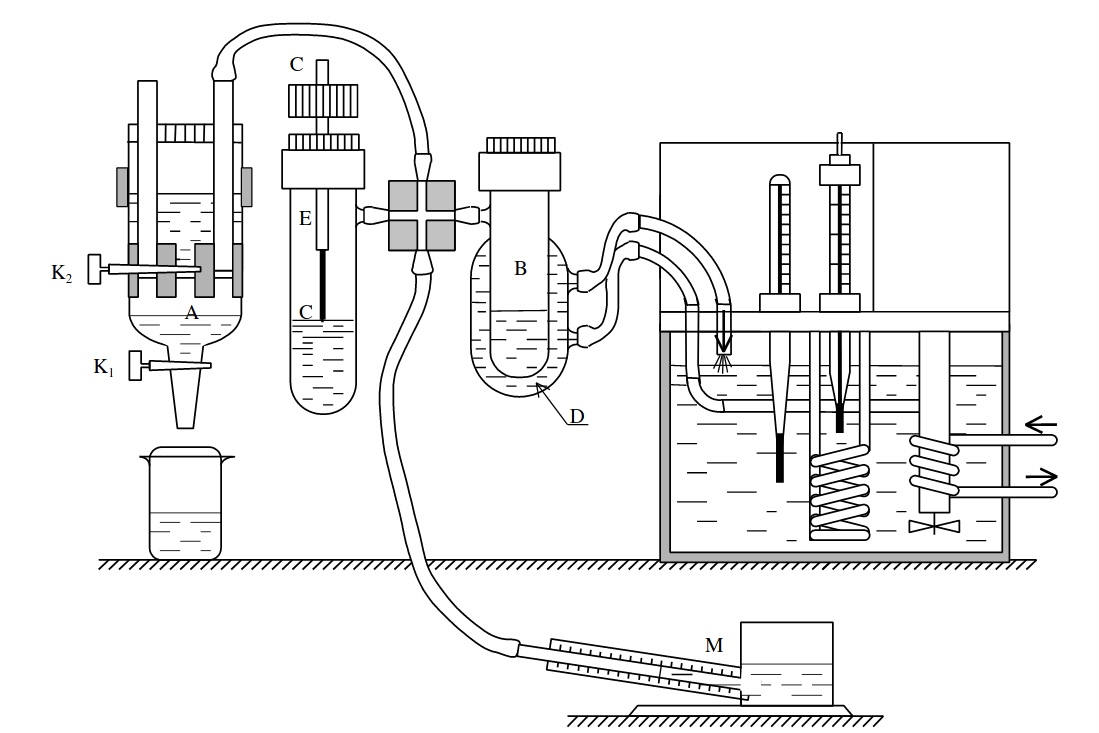
\includegraphics[width=\textwidth]{установка.jpg}
\end{center}
\caption{Схема установки}\label{установка}
\end{figure}

Схема экспериментальной установки представлена на рисунке \ref{установка}.
Тестовая жидкость (этиловый спирт) наливается в сосуд, через пробку в него входит полая металлическа игла. При создании достаточно разреженного воздуха в колбе пузырьки воздуха начинают пробулькивать, поверхностное натяжение измеряется по величине разряжения. Разряжение создается с помощью аспиратора, разность давлений измеряется спиртовым микроманометром.

Для стабилизации температуры через рубашку колбы с исследуемой жидкостью прогоняется вода из термостата. Из-за большой теплопроводности трубки температура в разных частях трубки заметно различна и ввиду теплового расширения поднимается уровень жидкости при изменении температуры. Поэтому при температурном измерениии кончик иглы опускают до самого дна сосуда, тогда:
\begin{equation}\label{погружение}
\Delta P = P - \rho g h
\end{equation}
$\rho$ - плотность жидкости, $h$ - высота погружения иглы.

\newpage

\section{Результаты измерений и обработка данных}

\subsection*{Табличные значения}

$$\sigma_{спирт} = (22.75 \pm 0.01) \ мН/м$$
$$\rho_{дист.вод} = (1.00 \pm 0.01) \ г/см^3$$
$$g = (9.81 \pm 0.01) \ м/с^2$$

\subsection*{Диаметр иглы}

Сначала определим диаметр иглы с помощью формулы (\ref{лаплас}). Разность давлений будем измерять несколько раз, принимая во внимание случайную погрешность и погрешность прибора.

\begin{table}[ht!]
	\centering
	\begin{tabular}{rrrrr}
\toprule
\midrule
43 & 43 & 44 & 43 & 43 \\
\bottomrule
\end{tabular}

	\caption{Показания микроманометра для спирта}
\end{table}

Связь измеряемого давления $P$ с отсчётом делений по шкале N:

$$P[Па] = 9.8067 \cdot N \cdot K,$$
где $K = 0.2$ — угловой коэффициент.

В итоге по формуле (\ref{лаплас}):

\begin{equation}\label{d_спирт}
	d_{спирт} = (1.084 \pm 0.016) \ мм
\end{equation}

А с помощью микроскопа:

\begin{equation}\label{d_микр}
	d_{микр} = (0.90 \pm 0.05) \ мм
\end{equation}

\subsection*{Глубина погружения}

Определим разность давлений $P_1$, когда игла лишь касается поверхности воды:

% \begin{table}[ht!]
% 	\centering
% 	\begin{tabular}{rrrrr}
\toprule
\midrule
118 & 118 & 118 & 119 & 119 \\
\bottomrule
\end{tabular}

% 	\caption{Показания микроманометра у поверхности воды}
% \end{table}

\begin{equation}\label{P1}
P_1 = (230.1 \pm 1.4) \ Па
\end{equation}

И расстояние от некоторой фиксированной точки до поверхности:

$$h_1 = (2.0 \pm 0.1) \ см$$

Теперь утопим иглу до предела (между концом иглы и дном необходимо оставить небольшой зазор, чтобы образующийся пузырёк не касался дна) и проделаем тоже самое:

% \begin{table}[ht!]
% 	\centering
% 	\begin{tabular}{rrrrr}
\toprule
\midrule
201 & 202 & 202 & 202 & 202.5 \\
\bottomrule
\end{tabular}

% 	\caption{Показания микроманометра у дна воды}
% \end{table}

\begin{equation}\label{P2}
	P_2 = (392.4 \pm 1.4) \ Па
\end{equation}
$$h_2 = (0.3 \pm 0.1) \ см$$

В итоге по формуле (\ref{погружение}):

\begin{equation}\label{h_теор}
	\Delta h_{теор} = \dfrac{P_2 - P_1}{\rho \cdot g} = (1.654 \pm 0.026) \ см
\end{equation}

И с помощью линейки:

\begin{equation}\label{h_лин}
	\Delta h_{лин} = (1.70 \pm 0.14) \ см
\end{equation}

\subsection*{Температурная зависимость}

Снимем температурную зависимость $N(T)$ показаний микроманометра дистиллированной воды:

\begin{table}[ht!]
	\centering
	\begin{tabular}{rrrrrr}
\toprule
$T$, $^\circ C$ & $N_1$ & $N_2$ & $N_3$ & $N_4$ & $N_5$ \\
\midrule
25.1 & 204.0 & 204.0 & 204.0 & 203.5 & 204.0 \\
30.3 & 202.5 & 202.0 & 202.5 & 202.5 & 202.5 \\
35.2 & 200.5 & 201.0 & 200.5 & 200.5 & 201.0 \\
40.2 & 198.5 & 199.0 & 199.0 & 199.0 & 199.5 \\
45.2 & 198.0 & 198.0 & 198.0 & 198.0 & 198.0 \\
50.2 & 196.5 & 197.5 & 196.5 & 197.0 & 197.0 \\
55.2 & 194.5 & 195.0 & 195.0 & 195.0 & 195.0 \\
60.1 & 193.0 & 193.0 & 192.5 & 193.0 & 193.0 \\
\bottomrule
\end{tabular}

	\caption{Показания микроманометра для дистиллированной воды}
\end{table}

По формулам (\ref{лаплас}) и (\ref{погружение}) рассчитаем величину коэффициента поверхностного натяжения воды $\sigma(T)$, используя значение диаметра иглы (\ref{d_спирт}), полученное при измерениях на спирте, и значение $\rho g \Delta h_{теор} = P_2 - P_1$, полученное при измерении глубины погружения (\ref{P1}) и (\ref{P2}):

$$\sigma = (P - \rho g \Delta h_{теор}) \cdot \dfrac{d_{спирт}}{4} $$

\begin{table}[ht!]
	\centering
	\begin{tabular}{rrr}
\toprule
$T$, $^\circ C$ & $\sigma$, $мН/м$ & $\sigma_{\sigma}$, $мН/м$ \\
\midrule
25.1 & 63.4 & 1.1 \\
30.3 & 62.6 & 1.1 \\
35.2 & 61.7 & 1.1 \\
40.2 & 60.8 & 1.1 \\
45.2 & 60.3 & 1.1 \\
50.2 & 59.7 & 1.1 \\
55.2 & 58.7 & 1.1 \\
60.1 & 57.6 & 1.0 \\
\bottomrule
\end{tabular}

	\caption{Коэффициент поверхностного натяжения}
\end{table}

\newpage

% \subsection*{Температурная зависимость на графике}

\begin{figure}[h!]
\begin{center}
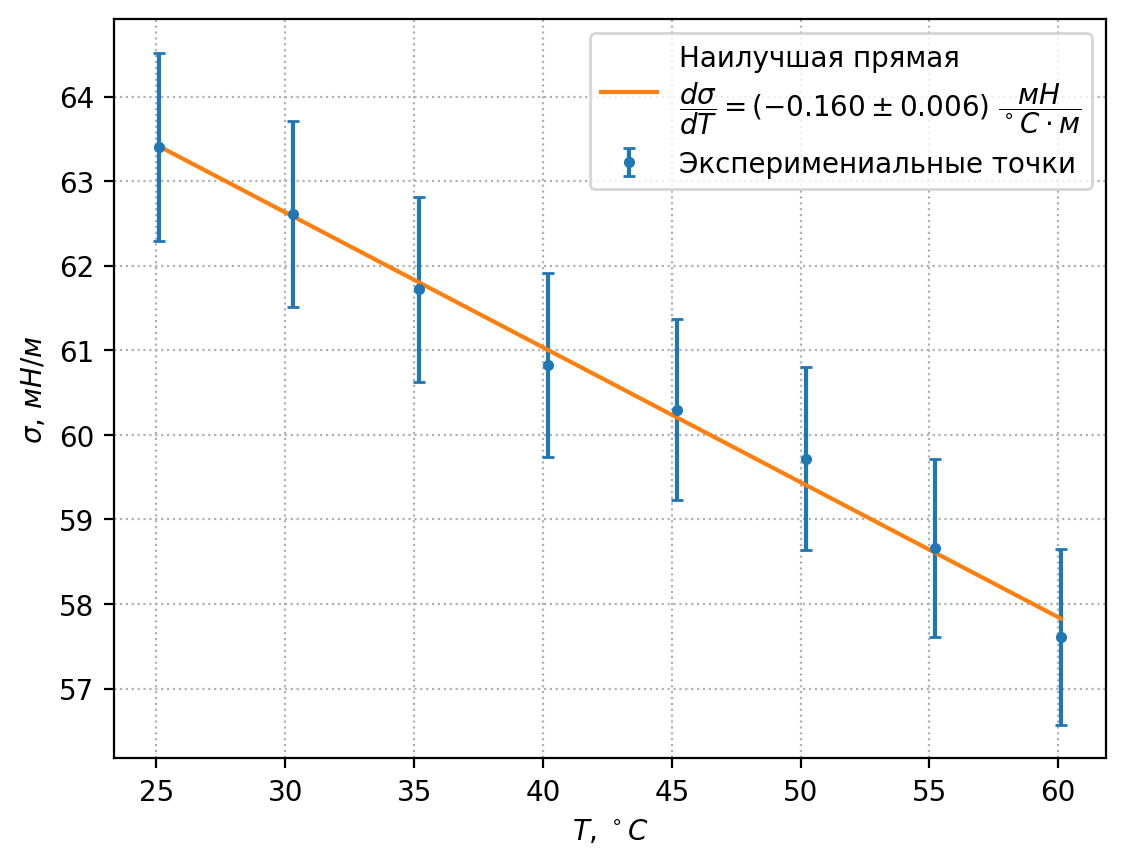
\includegraphics[width=0.875\textwidth]{8.png}
\end{center}
\caption{$\sigma(T)$}\label{sigma(T)}
\end{figure}

\begin{figure}[h!]
\begin{center}
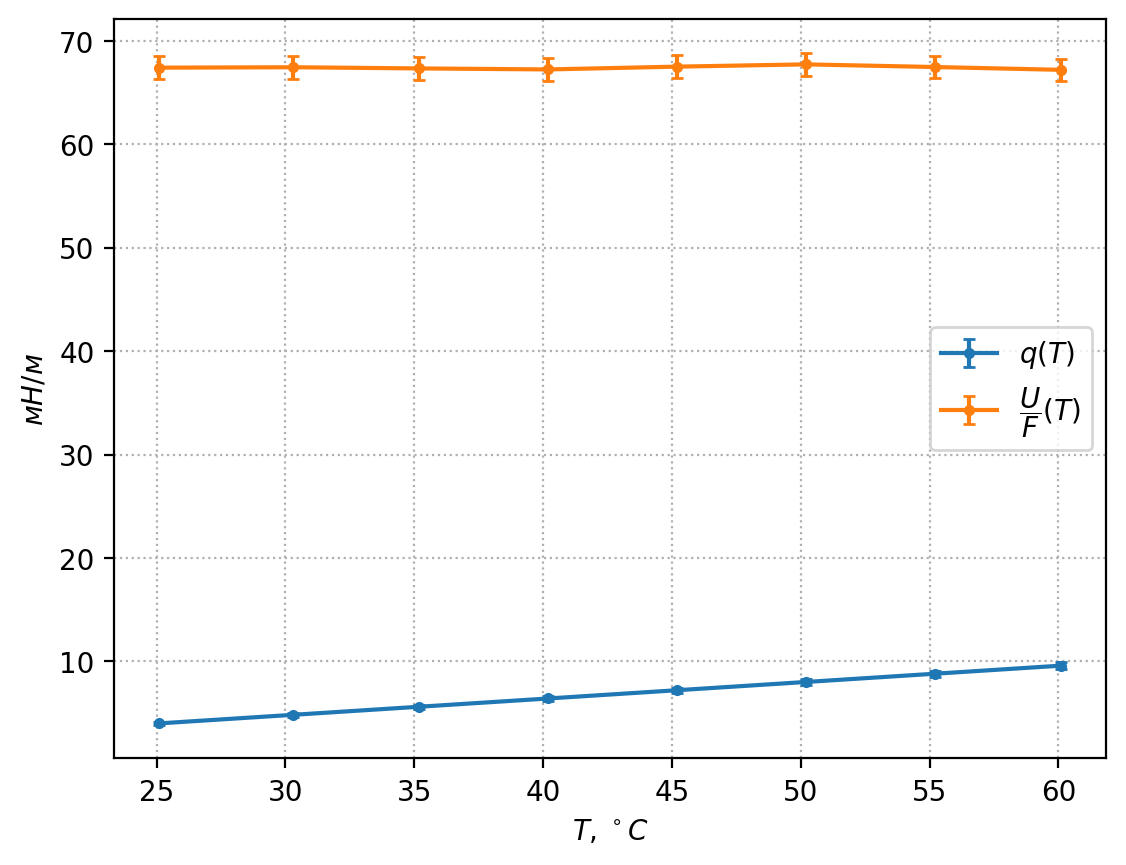
\includegraphics[width=0.875\textwidth]{9.png}
\end{center}
\caption{Теплота образования и поверхностная энергия}\label{W(T)}
\end{figure}

\section{Обсуждение результатов}

Значение диаметра иглы (\ref{d_спирт}), измеренное с помощью коэффициента вязкости спирта, близко к измеренному с помощью микроскопа (\ref{d_микр}), но в пределах погрешности значения не совпадают. Это можно объяснить тем, что игла была деформирована. В зависимости от положения иглы относительно линейки диаметр менялся. С помощью микроскопа был зафиксирован ее диаметр в самом узком месте.

Значение глубины погружения (\ref{h_теор}), измеренное с помощью разницы давлений, в пределах погрешности совпало с измеренным с помощью линейки (\ref{h_лин}).

Получена температурная зависимость коэффициента поверхностного натяжения (рис. \ref{sigma(T)}).

Вычислены зависимости теплоты образования единицы поверхности жидкости от температуры и поверхностной энергии единицы площади от температуры, постоянство второй из них подтверждается теоретически (рис. \ref{W(T)}).

\end{document}